\documentclass[12pt,spanish]{article}
\usepackage[spanish]{babel}
\usepackage{graphicx}
\usepackage{multirow}
\usepackage[hidelinks]{hyperref}
\usepackage{caption}
\usepackage{multirow}
\usepackage{multicol}
\usepackage[outputdir=build]{minted}
\usepackage{float}
\usepackage{array}
\graphicspath{ {../img/} {../../LaTeX/img/} {/home/csp98/latex/img/}}
\selectlanguage{spanish}
\usepackage[utf8]{inputenc}
\usepackage{graphicx}
\usepackage[a4paper,left=3cm,right=2cm,top=2.5cm,bottom=2.5cm]{geometry}
\newtheorem{ppio}{Principio }
\makeindex

\begin{document}
\begin{titlepage}

\newlength{\centeroffset}
\setlength{\centeroffset}{-0.5\oddsidemargin}
\addtolength{\centeroffset}{0.5\evensidemargin}
\thispagestyle{empty}

\noindent\hspace*{\centeroffset}
\begin{minipage}{\textwidth}

\centering
\includegraphics[width=0.9\textwidth]{logo_ugr.jpg}\\[1.4cm]

\textsc{ \Large Algorítmica\\[0.2cm]}
\textsc{GRADO EN INGENIERÍA INFORMÁTICA}\\[1cm]

{\Huge\bfseries Ejercicio de clase\\}
\noindent\rule[-1ex]{\textwidth}{3pt}\\[3.5ex]
{\large\bfseries Búsqueda ternaria}
\end{minipage}

\vspace{1.5cm}
\noindent\hspace*{\centeroffset}
\begin{minipage}{\textwidth}
\centering

\textbf{Autores}\\ {Carlos Sánchez Páez}\\[2.5ex]
\includegraphics[width=0.3\textwidth]{etsiit_logo.png}\\[0.1cm]
\vspace{1.5cm}
\includegraphics[width=0.5\textwidth]{decsai.jpg}\\[0.1cm]
\vspace{1cm}
\textsc{Escuela Técnica Superior de Ingenierías Informática y de Telecomunicación}\\
\vspace{1cm}
\textsc{Curso 2017-2018}
\end{minipage}
\end{titlepage}
\tableofcontents
\thispagestyle{empty}
\listoftables
\listoffigures
\newpage
\setcounter{page}{1}

\section{Enunciado}
\large{Realizar un estudio empírico para determinar si es preferible utilizar la búsqueda binaria o la búsqueda ternaria comentada en clase (ambos algoritmos son de orden logarítmico, pero sus constantes ocultas son diferentes).}

\section{Resolución}

\subsection{Metodología}
Para resolver el ejercicio, ejecutaremos 25 veces cada código con tamaños de problema ascendentes mediante un \textcolor{blue!50}{\hyperref[script]{script}}.
Después, estudiaremos empíricamente su eficiencia y hallaremos el valor de sus constantes ocultas (eficiencia híbrida). 

\begin{table}[H]
\centering
\begin{tabular}{|c|c|c|c|}
\hline
\textbf{Algoritmo} & \textbf{Tamaño inicial} & \textbf{Tamaño final} & \textbf{Incremento}\\
\hline
Búsqueda Binaria & & &\\
& 100.000.000 & 340.000.000 & 10.000.000\\
Búsqueda Ternaria & & &\\
\hline
\end{tabular}
\caption{Tamaños para la ejecución}
\end{table}

\subsection{Resultados obtenidos}
\begin{table}[H]
\centering
\begin{tabular}{|c|c|c|}
\hline
\textbf{Tamaño del problema} & \textbf{Búsqueda Binaria} & \textbf{Búsqueda Ternaria}\\
\hline

\end{tabular}
\caption{Tiempos obtenidos (seg)}
\end{table}

\subsection{Cálculo de la constante oculta}
Realizamos una regresión mediante \emph{gnuplot} para averiguar la constante:
\begin{table}[H]
\begin{tabular}{|c|c|c|}
\hline
\textbf{Algoritmo} & \textbf{Valor de la constante oculta} & \textbf{Porcentaje de error}\\
\hline
Búsqueda Binaria & & \\
\hline
Búsqueda Ternaria & & \\
\hline
\end{tabular}
\caption{Bondad del ajuste}
\end{table}

\subsection{Gráficas}

\begin{figure}[H]
%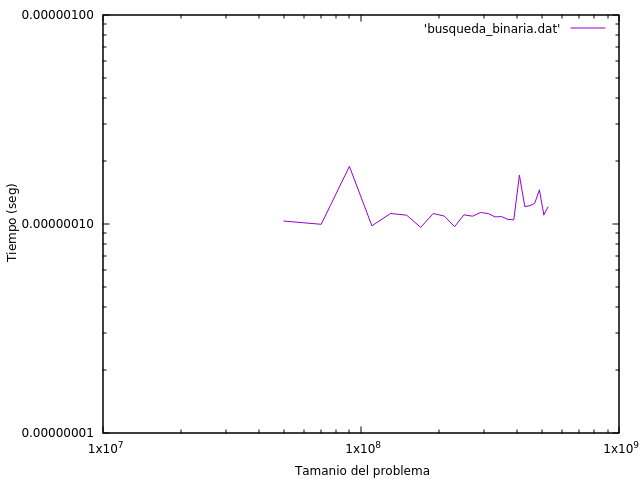
\includegraphics[scale=0.75]{empirica_binaria.png}
\caption{Eficiencia empírica. Búsqueda binaria}
\end{figure}

\begin{figure}[H]
%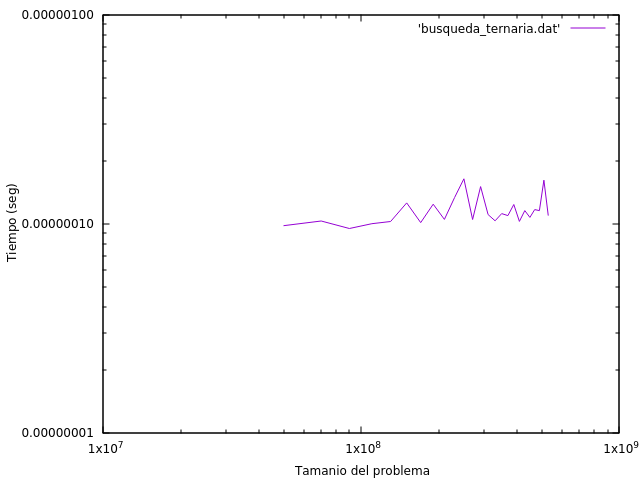
\includegraphics[scale=0.75]{empirica_ternaria.png}
\caption{Eficiencia empírica. Búsqueda ternaria}
\end{figure}

\begin{figure}[H]
%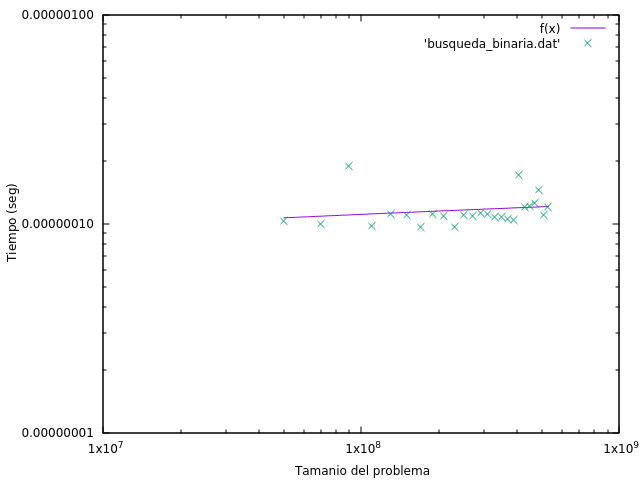
\includegraphics[scale=0.75]{hibrida_binaria.png}
\caption{Eficiencia híbrida. Búsqueda binaria}
\end{figure}

\begin{figure}[H]
%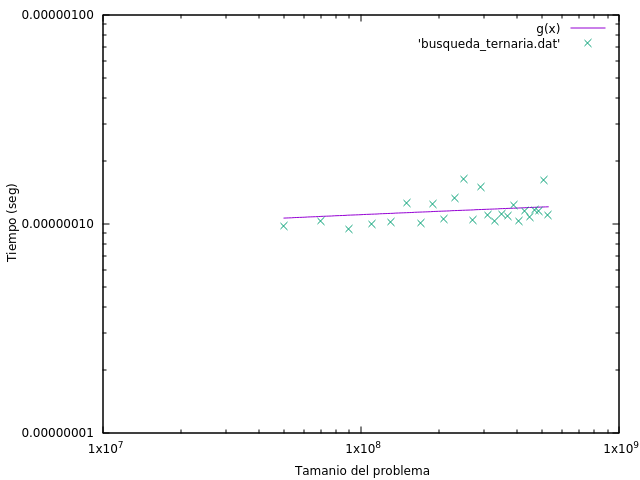
\includegraphics[scale=0.75]{hibrida_ternaria.png}
\caption{Eficiencia híbrida. Búsqueda ternaria}
\end{figure}

\subsection{Conclusiones}

\newpage
\subsection{Anexo:Algoritmos desarrollados}

\subsubsection{Búsqueda binaria}

\inputminted[linenos, fontsize=\footnotesize]{c++}{busqueda_binaria.cpp}

\newpage
\subsubsection{Búsqueda ternaria}

\inputminted[linenos, fontsize=\footnotesize]{c++}{busqueda_ternaria.cpp}


\subsubsection{Script para múltiples ejecuciones}
\label{script}

\inputminted[linenos, fontsize=\footnotesize]{bash}{individual.sh}

\subsubsection{Script de \emph{gnuplot}}

\inputminted[linenos, fontsize=\footnotesize]{bash}{gnuplot.sh}

\subsubsection{Script automatizado}

\inputminted[linenos, fontsize=\footnotesize]{bash}{all.sh}

\end{document}
